\documentclass[11pt,a4paper]{article}
\usepackage[utf8]{inputenc}
\usepackage[margin=0.7in,top=0.6in,bottom=0.6in]{geometry}
\usepackage{xcolor}
\usepackage{setspace}
\usepackage{tabularx}
\usepackage{tikz}
\usepackage[hidelinks]{hyperref}

% --- Brand Typography System ---
\usepackage[scaled=0.92]{helvet}
\renewcommand{\familydefault}{\sfdefault}

% --- Corporate Palette ---
\definecolor{SolidBlack}{HTML}{000000}
\definecolor{PureWhite}{HTML}{FFFFFF}
\definecolor{LinkBlue}{HTML}{0066CC}
\definecolor{CorporateNavy}{HTML}{0A192F}
\definecolor{SlateGray}{HTML}{4A5568}
\definecolor{LightSlate}{HTML}{F8FAFC}
\definecolor{BorderGray}{HTML}{CBD5E1}

\color{SolidBlack}
\pagecolor{PureWhite}
\pagestyle{empty}

\setstretch{1.15}
\setlength{\parindent}{0pt}
\setlength{\parskip}{0pt}

\begin{document}

% --- TOP LANYARD HOLE CUTOUT GUIDE ---
\begin{center}
    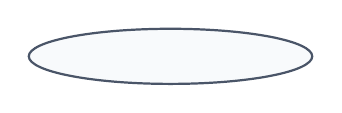
\begin{tikzpicture}
        \draw[fill=LightSlate, draw=SlateGray, line width=0.8pt] (0,0) ellipse (1.8cm and 0.35cm);
    \end{tikzpicture}
\end{center}

\vspace{0.2cm}

% --- CORPORATE METADATA TOP BAR ---
\begin{tabularx}{\textwidth}{@{} X >{\raggedleft\arraybackslash}X @{}}
    \textsf{\scriptsize\bfseries\color{LinkBlue} CREDENTIAL ID: MCH-2026-EXEC-001} & \textsf{\scriptsize\bfseries\color{CorporateNavy} OFFICIAL LAUNCH EVENT} \\
    \textsf{\tiny\color{SlateGray} AUTHENTICATED ACCESS PASS} & \textsf{\tiny\color{SlateGray} NAIROBI, KENYA} \\
\end{tabularx}

\vspace{0.4cm}

% --- CLEAN BRAND HEADER ---
\begin{tabularx}{\textwidth}{@{} X >{\raggedleft\arraybackslash}X @{}}
    {\fontsize{48}{54}\sffamily\bfseries\color{CorporateNavy} Muncheez\color{LinkBlue}{\textbf{.}}} & 
    \begin{raggedleft}
        {\fontsize{13}{16}\sffamily\bfseries\color{CorporateNavy} DIGITAL SOFTWARE MARKETPLACE} \\[0.05cm]
        {\fontsize{10}{13}\sffamily\bfseries\color{LinkBlue}\uppercase{Logistics Infrastructure}}
    \end{raggedleft} \\
\end{tabularx}

\vspace{0.5cm}
% Asymmetric Divider

\begin{tikzpicture}
    \draw[line width=1.5pt, color=CorporateNavy] (0,0) -- (\textwidth-1.5cm, 0);
    \draw[line width=1.5pt, color=LinkBlue] (\textwidth-1.5cm,0) -- (\textwidth, 0);
\end{tikzpicture}

\vspace{1.2cm}

% --- EXECUTIVE ATTENDEE NAME BLOCK (INLINE HORIZONTAL FOCUS) ---
\textsf{\xs\bfseries\color{LinkBlue}\uppercase{Executive Delegate}} 

\vspace{0.3cm}

{\fontsize{52}{58}\sffamily\bfseries\color{CorporateNavy} Dean Ndere}
% Note: If adding a long third name (e.g. Fiona Njaga Kariuki), drop the 3rd name directly below:
% \\[0.15cm] {\fontsize{38}{44}\sffamily\bfseries\color{CorporateNavy} Kariuki}

\vspace{1.2cm}

% --- RESTRUCTURED MID-PAGE CONTENT & PROMINENT QR SECTION ---
\color{BorderGray}\hrule height 1pt
\vspace{0.6cm}

\begin{tabularx}{\textwidth}{@{} X !{\color{BorderGray}\vrule width 1pt} p{5.5cm} @{}}
    % LEFT SIDE: TITLE & DETAILS
    \begin{raggedright}
        \textsf{\xs\bfseries\color{SlateGray}\uppercase{Corporate Title}} \\[0.15cm]
        {\fontsize{22}{26}\sffamily\bfseries\color{CorporateNavy} Chief Executive Officer} \\[0.1cm]
        {\fontsize{14}{17}\sffamily\color{SlateGray} Muncheez Technologies Inc.}
        
        \vspace{0.8cm}
        
        \textsf{\xs\bfseries\color{SlateGray}\uppercase{Access Level \& Zone}} \\[0.15cm]
        {\fontsize{15}{18}\sffamily\bfseries\color{CorporateNavy} All Areas / Keynote Stage} \\[0.1cm]
        {\textsf{\small\color{LinkBlue}\bfseries Full Executive Clearance}}
    \end{raggedright}
    & 
    % RIGHT SIDE: PROMINENT QR CODE PANEL
    \begin{center}
        \textsf{\tiny\bfseries\color{CorporateNavy} SCAN FOR GATE VERIFICATION} \\[0.2cm]
        
        
\begin{tikzpicture}[x=1.6mm, y=1.6mm]
            \draw[fill=PureWhite, draw=BorderGray, line width=0.8pt, rounded corners=1mm] (-1.5,-1.5) rectangle (26.5,26.5);
            
            % Dense noise grid
            \foreach \x in {0,...,24} {
                \foreach \y in {0,...,24} {
                    \pgfmathparse{mod(\x*\y + \x*7 + \y*3, 7) < 3 ? 1 : 0}
                    \ifnum\pgfmathresult=1
                        \draw[fill=CorporateNavy, draw=none] (\x,\y) rectangle (\x+1,\y+1);
                    \fi
                }
            }
            
            % Position Boxes
            \draw[fill=PureWhite, draw=none] (0,18) rectangle (7,25);
            \draw[fill=CorporateNavy, draw=none] (0,18) rectangle (7,25);
            \draw[fill=PureWhite, draw=none] (1,19) rectangle (6,24);
            \draw[fill=CorporateNavy, draw=none] (2,20) rectangle (5,23);

            \draw[fill=PureWhite, draw=none] (18,18) rectangle (25,25);
            \draw[fill=CorporateNavy, draw=none] (18,18) rectangle (25,25);
            \draw[fill=PureWhite, draw=none] (19,19) rectangle (24,24);
            \draw[fill=CorporateNavy, draw=none] (20,20) rectangle (23,23);

            \draw[fill=PureWhite, draw=none] (0,0) rectangle (7,7);
            \draw[fill=CorporateNavy, draw=none] (0,0) rectangle (7,7);
            \draw[fill=PureWhite, draw=none] (1,1) rectangle (6,6);
            \draw[fill=CorporateNavy, draw=none] (2,2) rectangle (5,5);

            \draw[fill=PureWhite, draw=none] (16,3) rectangle (21,8);
            \draw[fill=CorporateNavy, draw=none] (16,3) rectangle (21,8);
            \draw[fill=PureWhite, draw=none] (17,4) rectangle (20,7);
            \draw[fill=CorporateNavy, draw=none] (18,5) rectangle (19,6);
        \end{tikzpicture} \\[0.2cm]
        \textsf{\tiny\ttfamily\color{SlateGray} PASS: DEAN-NDERE-2026}
    \end{center} \\
\end{tabularx}

\vspace{0.6cm}
\color{BorderGray}\hrule height 1pt

\vfill

% --- FULL WIDTH LINEAR BARCODE FOOTER ---
\begin{center}
    \textsf{\tiny\bfseries\color{CorporateNavy} AUTHENTICATED SYSTEM BARCODE} \\[0.15cm]
    
\begin{tikzpicture}[x=1.1mm, y=1mm]
        \foreach \x/\w in {
            0/0.4, 1/1.2, 3/0.4, 4/0.8, 6/1.6, 9/0.4, 10/1.2, 12/0.8, 14/0.4, 15/1.6, 
            18/0.4, 19/0.8, 21/1.2, 23/0.4, 25/1.6, 28/0.8, 30/0.4, 31/1.2, 33/1.6, 
            36/0.4, 37/0.8, 39/1.2, 41/0.4, 43/1.6, 46/0.8, 48/0.4, 49/1.2, 51/0.4, 
            53/1.6, 56/0.4, 57/1.2, 59/0.8, 61/0.4, 62/1.6, 65/0.8, 67/0.4, 68/1.2,
            71/0.4, 72/1.6, 75/0.8, 77/0.4, 78/1.2, 80/0.8, 82/0.4, 83/1.6
        } {
            \draw[fill=CorporateNavy, draw=none] (\x,0) rectangle (\x+\w, 10);
        }
    \end{tikzpicture} \\[0.1cm]
    \textsf{\tiny\ttfamily\color{SlateGray} MCH*8920-EXEC-DEAN-NDERE*2026}
\end{center}

\vspace{0.5cm}

% --- BOTTOM EXECUTIVE ROLE BANNER ---

\begin{tikzpicture}
    \node[fill=CorporateNavy, text=PureWhite, minimum width=\textwidth, minimum height=1.6cm, inner sep=0pt] at (0,0) {
        {\fontsize{22}{26}\sffamily\bfseries CHIEF EXECUTIVE OFFICER \hspace{0.4cm}\textperiodcentered\hspace{0.4cm} ALL ACCESS}
    };
\end{tikzpicture}

\end{document}
